\section{Arquitectura capa de negocio}
{Esta capa, es la capa de arquitectura del proyecto orientada al negocio, aquí se plasma el enfoque organizacional, las reglas que regirán el negocio y las entidades que representan el sistema, permitiendo obtener de forma optima los roles y actores que aquí se desempeñan \cite{archimate}.}

	\subsection{Punto de vista de organización}
	{ El punto de vista organizacional esta enfocado a la estructura interna de la empresa, departamento o entidad organizacional, este refleja de forma jerárquica el nivel de los actores y roles que aquí interactúan \cite{archimate}.\\
		
		\textbf{Modelo}\\
		\begin{figure}[H]
			\centering
			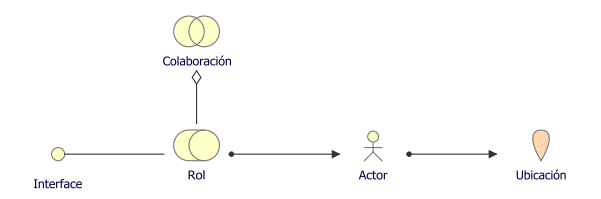
\includegraphics[width=0.8\linewidth]{development/organizacion.png}
			\caption{Metamodelo de Organización}
		\end{figure}
		\begin{center}
			\textbf{Fuente:} Colosoft E.U: Documento CasoColoSoft.
		\end{center}
	
		\textbf{Caso:} La organización se encuentra ubicada en la ciudad de Bogotá donde sus principales actores son:
		
		\begin{itemize}
			\item Tendero
			\item Consumidor
		\end{itemize}
		
		\begin{figure}[H]
			\centering
			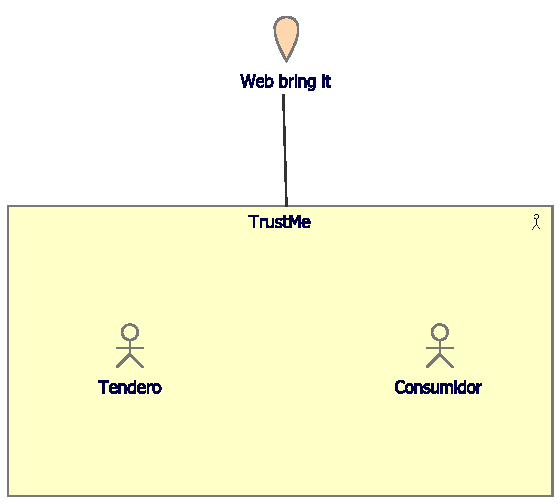
\includegraphics[width=0.6\linewidth]{development/negocio.pdf}
			\caption{Organización}
		\end{figure}
		\begin{center}
			\textbf{Fuente:} Propia.
		\end{center}
	}
	
	\subsection{Punto de vista de cooperación de actor}
	{Se  basa en mostrar el número total de actores los cuales influyen en el negocio y las cooperaciones de fuentes externas, mostrando la forma en que se relacionan entre sí \cite{archimate}.\\
	\newpage
		
		\textbf{Modelo}\\
		\begin{figure}[H]
			\centering
			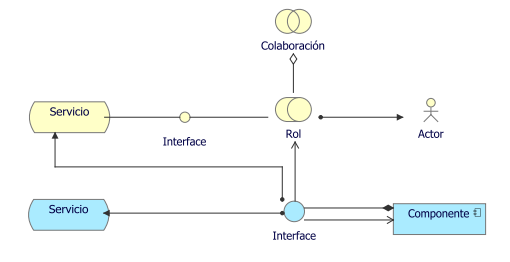
\includegraphics[width=0.8\linewidth]{development/cooperacionactor.png}
			\caption{Metamodelo de cooperación de actor}
		\end{figure}
		\begin{center}
			\textbf{Fuente:} Colosoft E.U: Documento CasoColoSoft.
		\end{center}
		\hfill \break
		
		\textbf{Caso:} Los principales actores y su relación con el negocio son:
		
		\begin{itemize}
			\item \textbf{Tendero:} persona quien vende los productos al fiado en la aplicación.
			
			\item \textbf{Consumidor:} persona quien acepta una deuda por fiar en la aplicación.
			
			\item \textbf{Administrador:} Ente encargado de administrar los demás perfiles en la aplicación.
			
		\end{itemize}
		
		\begin{figure}[H]
			\centering
			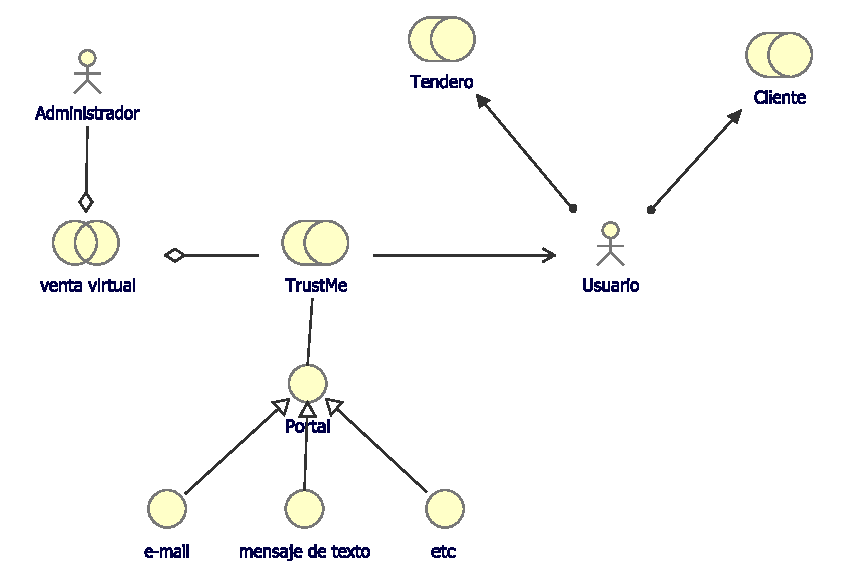
\includegraphics[width=0.8\linewidth]{development/cooperacionactor.pdf}
			\caption{Cooperación de actor}
		\end{figure}
		\begin{center}
			\textbf{Fuente:} Propia.
		\end{center}
	}
	
	\subsection{Punto de vista de función de negocio}
	{ En el punto de vista de función de negocio se muestra al detalle el funcionamiento de la organización, aquí se brinda un aspecto generalizado de las actividades primarias que se ejecutan y permite representar la estabilidad de la aplicación \cite{archimate}.\\
		
		\textbf{Modelo}\\
		\begin{figure}[H]
			\centering
			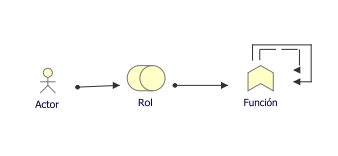
\includegraphics[width=0.6\linewidth]{development/funcion.png}
			\caption{Metamodelo de función de negocio}
		\end{figure}
		\begin{center}
			\textbf{Fuente:} Colosoft E.U: Documento CasoColoSoft.
		\end{center}
		
		\textbf{Caso:} En el negocio debe existir una persona dispuesta a ofertar sus productos al "fiado", el cual se gestionara por la app, luego un según actor quien se encuentre interesado pedirá fiado este, que será despachado hacia él.
		
		\begin{figure}[H]
			\centering
			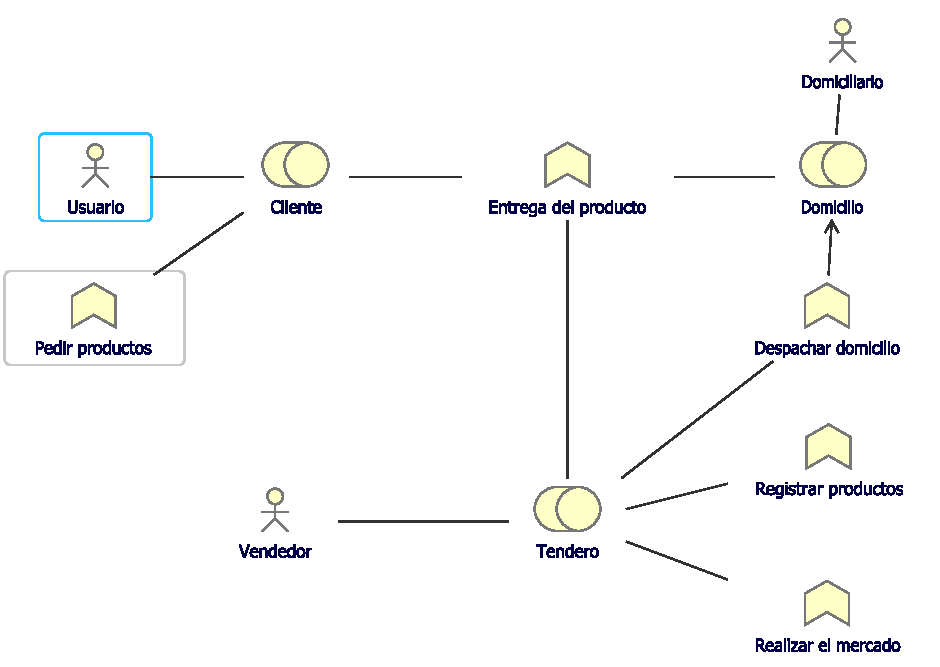
\includegraphics[width=0.8\linewidth]{development/funcion.pdf}
			\caption{Función de negocio}
		\end{figure}
		\begin{center}
			\textbf{Fuente:} Propia.
		\end{center}
	}
	
	\subsection{Punto de vista de proceso de negocio}
	{ El punto de vista del proceso de negocio, muestra una composición de alto nivel de los procesos encadenados en relación a los servicios que se ofrecen y la contribución de este con los productos de la empresa, permite una asignación de funciones a cada actor loas cuales definen su rol \cite{archimate}.\\
	\newpage
		
		\textbf{Modelo}\\
		\begin{figure}[H]
			\centering
			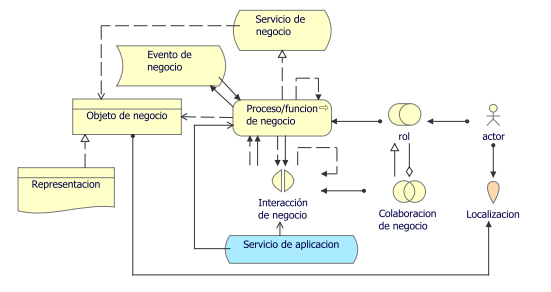
\includegraphics[width=0.8\linewidth]{development/proceso.png}
			\caption{Metamodelo de proceso de negocio}
		\end{figure}
		\begin{center}
			\textbf{Fuente:} Colosoft E.U: Documento CasoColoSoft.
		\end{center}
		\hfill \break
		
		\textbf{Caso:} Los procesos o actividades principales del proceso de negocio son:
		
		\begin{itemize}
			\item \textbf{Fiar - prestar:} Consiste en el evento de un tendero o persona, de dar a cuotas un producto o prestar un dinero.
			
			\item \textbf{Pedir prestado:} Consiste en el evento de solicitar un producto, el cual será pagado a cuotas.
			
		\end{itemize}
		
		Ambos eventos deberán ser procesados por la aplicación para su registro y gestión de los mismos.
		
		
		\begin{figure}[H]
			\centering
			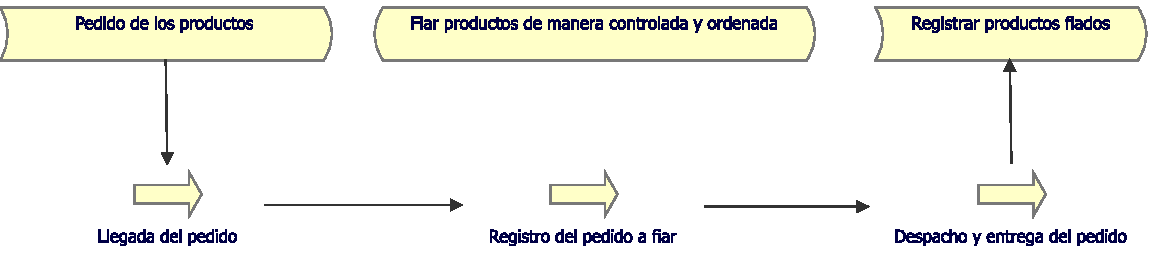
\includegraphics[width=0.8\linewidth]{development/proceso.pdf}
			\caption{Proceso de negocio}
		\end{figure}
		\begin{center}
			\textbf{Fuente:} Propia.
		\end{center}
	}
	
	\subsection{Cooperación de proceso de negocio}
	{ La cooperación de proceso de negocio muestra la relación entre los procesos del negocio con su entorno y sus respectivas dependencias \cite{archimate}.\\
		
		\textbf{Modelo}\\
		\begin{figure}[H]
			\centering
			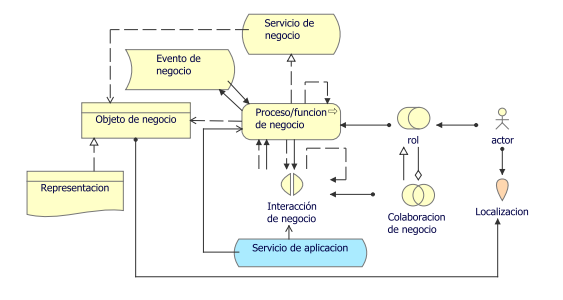
\includegraphics[width=0.8\linewidth]{development/cooperacionproceso.png}
			\caption{Metamodelo de cooperación de proceso de negocio}
		\end{figure}
		\begin{center}
			\textbf{Fuente:} Colosoft E.U: Documento CasoColoSoft.
		\end{center}
		\hfill \break
		
		\textbf{Caso:} Se especifica cuáles son los actores que influyen en los procesos, en este caso es la gestión de microcréditos (fiar).
		
		
		\begin{figure}[H]
			\centering
			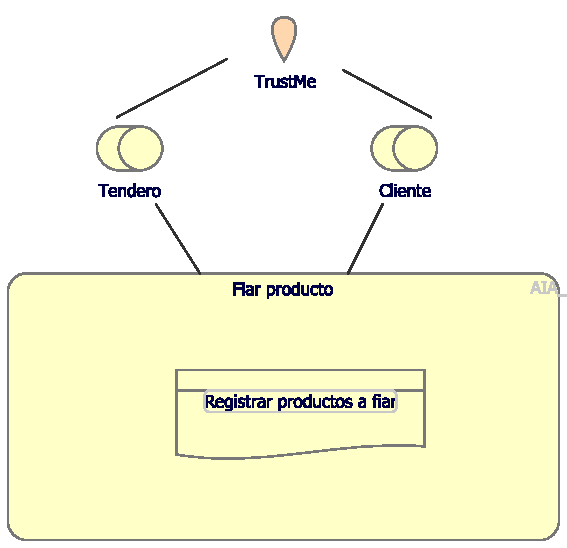
\includegraphics[width=0.6\linewidth]{development/cooperacionproceso.pdf}
			\caption{Cooperación de proceso de negocio}
		\end{figure}
		\begin{center}
			\textbf{Fuente:} Propia.
		\end{center}
		\hfill
	}
	
	\subsection{Punto de vista de producto}
	{ El producto muestra el valor que este mismo le ofrece a los clientes o a todas las partes que se encuentren involucradas en el proceso, se visualiza la composición de estos en términos de servicios y pueden utilizados para generar interfaces que ayudaran con su oferta \cite{archimate}.\\
	\newpage
		
		\textbf{Modelo}\\
		\begin{figure}[H]
			\centering
			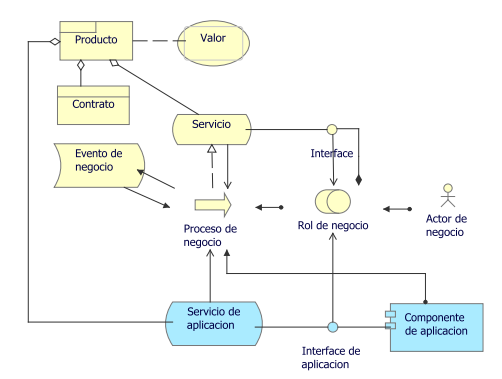
\includegraphics[width=0.8\linewidth]{development/producto.png}
			\caption{Metamodelo de producto}
		\end{figure}
		\begin{center}
			\textbf{Fuente:} Colosoft E.U: Documento CasoColoSoft.
		\end{center}
		\hfill \break
		
		\textbf{Caso:} En este caso el producto es la aplicación de gestión de préstamos, la cual brinda una plataforma confiable que genera cálculos totales de las deudas o préstamos previamente registrados.
	
		
		\begin{figure}[H]
			\centering
			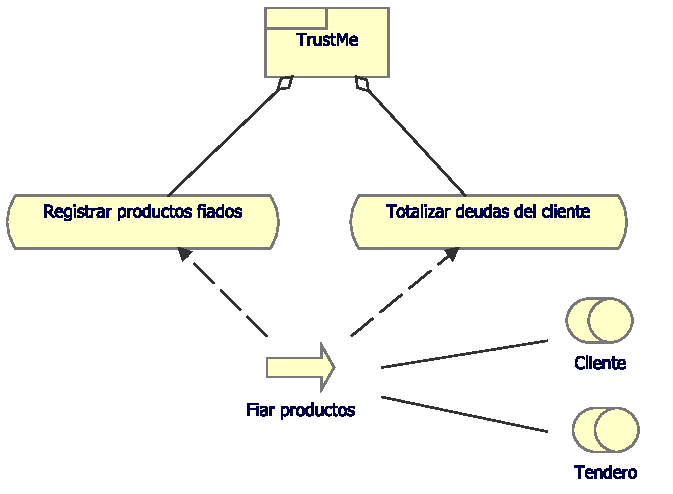
\includegraphics[width=0.8\linewidth]{development/producto.pdf}
			\caption{Producto}
		\end{figure}
		\begin{center}
			\textbf{Fuente:} Propia.
		\end{center}
	}